\documentclass{ximera}

\author{Paul Zachlin \and Anna Davis} \title{$\mathbb{R}^n$ and Subspaces of $\mathbb{R}^n$.} \license{CC-BY 4.0}

\renewcommand{\vec}[1]{{\bf #1}}
\newcommand{\RR}{\mathbb{R}}
\newcommand{\dfn}{\textit}
\newcommand{\dotp}{\cdot}
\pgfplotsset{compat=1.14}

\newtheorem{general}{Generalization}
\newtheorem{initprob}{Exploration Problem}
\usepackage{tikz-cd}
\usepackage{tikz-3dplot}

\begin{document}
\begin{abstract}
We define closure under addition and scalar multiplication, and we demonstrate how to determine whether a subset of vectors in $\RR^n$ is a subspace of $\RR^n$.
\end{abstract}

\maketitle

\section*{Closure}
% {\color{red}do we need this first paragraph?}
% In the module VSP-M-0003 we examined how to graphically represent the vectors in $\RR^n$ for $n=1, 2,$ or 3.  We were also introduced to thinking of elements of $\RR^n$ as ordered $n$-tuples $(x_1, x_2, \ldots, x_n)$, and later as $n \times 1$ matrices.  These representations are particularly important for $n>3$ when we are unable to represent vectors graphically.

% %In later modules, we learned about two operations that can be applied to vectors in $\RR^n$, namely, addition and scalar multiplication.  We also learned that these operations satisfy many nice properties.  In fact, these properties are what make $\RR^n$ a \emph{vector space}, as we will study in module VSP-M-0050.
% {\color{red}this is a pretty good opener...}
We are familiar with two operations that can be applied to vectors in $\RR^n$, namely, addition and scalar multiplication. We learned that addition and scalar multiplication satisfy many nice properties. (See Theorem \ref{th:vecproperties}) These properties give $\RR^n$ an algebraic structure, and make $\RR^n$ a \dfn{vector space}.  Before we can give a formal definition of a vector space we need to introduce the concept of \dfn{closure} under an operation.

%In this module, we study subsets of $\RR^n$ that are also vector spaces.  Such a subset of $\RR^n$ is called a \emph{subspace}.  In order to discuss subspaces, it is helpful to understand the concept of \emph{closure} of an operation.


 \begin{definition} 
  A set $V$ is said to be \emph{closed under addition} if for each element $\vec{u} \in V$ and $\vec{v} \in V$ the sum $\vec{u}+\vec{v}$ is also in $V$.
\end{definition}

% {\color{red}Can we change the last part to read, "the sum u+v is also in V"?  (sweep existence and uniqueness of the sum under the rug)  When we prove closure later we don't want to have to prove that the sum is unique... Same comment for the next definition.}   GOOD CORRECTIONS!


  \begin{definition} 
  A set $V$ is said to be \emph{closed under scalar multiplication} if for each element $\vec{v} \in V$  and for each scalar $c$ the product $c\vec{v}$ is also in $V$.
\end{definition}


\begin{example}
Let $E$ be the set of positive even integers.  Then $E$ is closed under addition, because the sum of two even integers is again an even integer.
\end{example}

\begin{example}
Let $D$ be the set of positive odd integers.  Then $D$ is not closed under addition, for the sum of two odd integers need not be an odd integer (in fact, it will always be even).
\end{example}

\begin{example} \label{ex:Q1}
Let $X_1$ be defined as follows.
$$X_1=\left\{\begin{bmatrix} x_1\\x_2\end{bmatrix} \in \mathbb{R}^2 : x_1 \ge 0, x_2 \ge 0 \right\}$$
In other words, $X_1$ is the set of vectors in $\mathbb{R}^2$ in the first quadrant (or on an axis on the boundary of the first quadrant). Show that $X_1$ is closed under addition, but $X_1$ is not closed under scalar multiplication.

% {\color{red} Ooops! I just saw that you wanted students to verify BOTH 3 and 4.  Feel free to remove my solution.}

\begin{explanation} Suppose $\vec{v}_1=\begin{bmatrix}a\\b\end{bmatrix}$ and $\vec{v}_2=\begin{bmatrix}c\\d\end{bmatrix}$ are in $X_1$.  This means that $a, b, c, d\geq 0$.  But then we have $a+c, b+d\geq 0$.  Therefore $\vec{v}_1+\vec{v}_2=\begin{bmatrix}a+c\\b+d\end{bmatrix}$ is also in $X_1$. We conclude that $X_1$ is closed under addition.

$X_1$ is not closed under scalar multiplication because $(-1)\vec{v}_1=\begin{bmatrix}-a\\-b\end{bmatrix}$ is not in $X_1$.

% In addition to an algebraic proof, it is instructive to consider this problem from a geometric perspective.  

The figure below helps us see that the sum of any two vectors in $X_1$ also lies in $X_1$, but any negative scalar multiple of a vector in $X_1$ does not lie in $X_1$.

\begin{center}
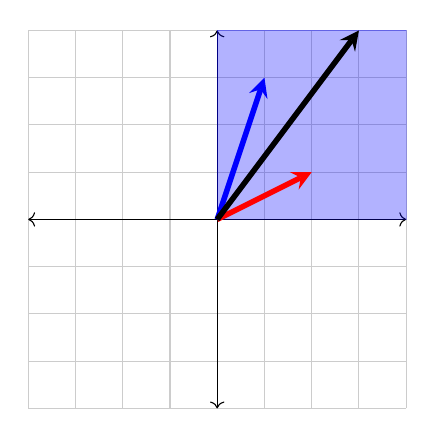
\begin{tikzpicture}[scale=0.6]
\draw[thin,gray!40] (-4,-4) grid (4,4);
  \draw[<->] (-4,0)--(4,0);
  \draw[<->] (0,-4)--(0,4);
  
  \filldraw[blue, opacity=0.3](0,0)--(4,0)--(4,4)--(0,4)--cycle;
\draw[line width=2pt,red,-stealth](0,0)--(2,1) ;

 % \fill[blue!40!white] (10,0) circle (0.2cm);
 \draw[line width=2pt,blue,-stealth](0,0)--(1,3) ;
 
 \draw[line width=2pt,-stealth](0,0)--(3,4); 
\end{tikzpicture}\quad
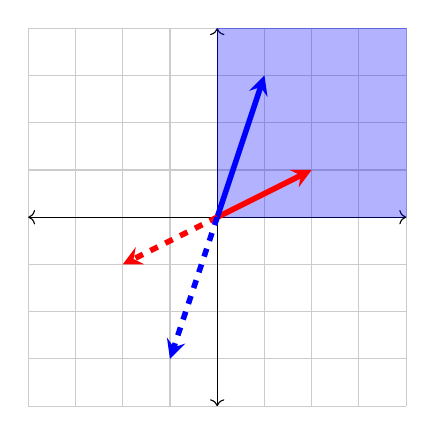
\begin{tikzpicture}[scale=0.6]
\draw[thin,gray!40] (-4,-4) grid (4,4);
  \draw[<->] (-4,0)--(4,0);
  \draw[<->] (0,-4)--(0,4);
  
  \filldraw[blue, opacity=0.3](0,0)--(4,0)--(4,4)--(0,4)--cycle;
\draw[line width=2pt,red,-stealth](0,0)--(2,1) ;
 \draw[line width=2pt,blue,-stealth](0,0)--(1,3) ;
 \draw[line width=2pt,red,dashed,-stealth](0,0)--(-2,-1) ;
 \draw[line width=2pt,blue,dashed,-stealth](0,0)--(-1,-3) ;

\end{tikzpicture}
\end{center}
\end{explanation}
\end{example}

\begin{example} \label{ex:Q1-3}
Let $X_1$ be as in Example \ref{ex:Q1}.  Let $X_3=\left\{\begin{bmatrix} x_1\\x_2\end{bmatrix} \in \mathbb{R}^2 : x_1 \le 0, x_2 \le 0 \right\}$.
In other words, $X_3$ is the set of vectors in $\RR^2$ in the third quadrant (or on an axis on the boundary of the third quadrant).  Now let 
$$Y = X_1 \bigcup X_3,$$ 
i.e., $Y$ is the set of vectors in $\RR^2$ that are either in the first quadrant, the third quadrant, or lie along one of the axes.  Then $Y$ is closed under scalar multiplication, but $Y$ is not closed under addition.
\begin{explanation} See if you can verify this claim on your own.  If not, watch the following video:

\end{explanation}

\end{example}

%See if you can verify the claims made in Examples \ref{ex:Q1} and \ref{ex:Q1-3} above.  If not, watch the following video:

 
\section*{$\RR^n$ as a Vector Space}

In module VEC-M-0030 we learned that vector addition and scalar multiplication in $\RR^n$ satisfy the following eight properties:

\begin{theorem}\label{th:vecproperties} The following properties hold for vectors ${\bf u}$, ${\bf v}$ and ${\bf w}$ in $\mathbb{R}^n$ and scalars $k$ and $p$.
\begin{enumerate}
  \item 
  Commutative Property of Addition:
  $\vec{u}+\vec{v}=\vec{v}+\vec{u}$
  \item 
  Associative Property of Addition:
  $(\vec{u}+\vec{v})+\vec{w}=\vec{u}+(\vec{v}+\vec{w})$
  \item 
  Existence of Additive Identity:
  $\vec{u}+\vec{0}=\vec{u}$
  \item 
  Existence of Additive Inverse:
  $\vec{u}+(-\vec{u})=\vec{0}$
  \item
  Distributive Property over Vector Addition:
  $k(\vec{u}+\vec{v})=k\vec{u}+k\vec{v}$
  \item
  Distributive Property over Scalar Addition:
  $(k+p)\vec{u}=k\vec{u}+p\vec{u}$
  \item 
  Associative Property for Scalar Multiplication:
  $k(p\vec{u})=(kp)\vec{u}$
  \item 
  Multiplication by 1:
  $1\vec{u}=\vec{u}$
  \end{enumerate}
\end{theorem}

  
  In addition, observe that $\RR^n$ is closed under addition and scalar multiplication.  (Why?)  The eight properties of vector operations, together with closure, constitute the criteria for a set with two operations to be considered a \dfn{vector space}.  $\RR^n$ is a vector space.  We will encounter other vector spaces later. Any vector space must be closed under both operations, and must satisfy the other eight properties in the list above.  We will see (in module VSP-M-0050, for instance) that there is a wide variety of sets, with a wide variety of operations, that are vector spaces (which is one of the reasons we study linear algebra).  As we shall see, these sets and their operations may look very different, but the behavior of the two operations makes them vector spaces.  For now, we simply focus on $\RR^n$.


\section*{Subspaces of $\RR^n$}

Now that we understand what it means for a set to be closed under addition and scalar multiplication, we are ready for the main definition of this module.

% {\color{blue} We now turn our attention to subsets of $\RR^n$ that are also vector spaces.  Such a subset of $\RR^n$ is called a \dfn{subspace}.  To prove that a subset of $\RR^n$ is a subspace, we would have to prove that the subset is a vector space in its own right.  This can be done by verifying the eight properties of vector addition and multiplication, and checking closure.  Fortunately, checking every property turns out to be unnecessary.  We will later prove that if a subset is closed under addition and scalar multiplication, then the eight properties of vector addition and scalar multiplication will automatically be satisfied by virtue of closure and the fact that the given set is a subset of $\RR^n$.  While we don't yet have the proof of this, we present this idea as a definition.}

% \begin{definition}[Two-part Subspace Test]\label{def:subspacetest} Suppose that $V$ is a subset of $\RR^n$ that is closed under addition and closed under scalar multiplication.  Then $V$ is a \dfn{subspace} of $\RR^n$.
% \end{definition} 

\begin{definition}\label{def:subspace} Suppose that $V$ is a subset of $\RR^n$ that is closed under addition and closed under scalar multiplication.  Then $V$ is a \dfn{subspace} of $\RR^n$.
\end{definition}
We use the term \dfn{subspace} because it turns out that any subset of a vector space which is closed under both addition and scalar multiplication is also a vector space.  In other words, in addition to satisfying the properties of closure, a subspace will automatically satisfy the eight other vector space properties listed in \ref{th:vecproperties}.  We will prove this in VSP-M-0050.

\begin{example} \label{y-axis_subspace}
Let $V$ be the set of vectors in $\RR^3$ on the $y-$axis.  Then $V$ is a subspace of $\RR^3$.  

\begin{explanation}
To verify this, note that any vector in $V$ is of the form $\begin{bmatrix}0\\y\\0 \end{bmatrix}$.  If we multiply such a vector by a scalar $c$, we get a vector of the form $\begin{bmatrix}0\\cy\\0 \end{bmatrix}$, which is clearly still in $V$.  This proves $V$ is closed under scalar multiplication.  Next, note that $\begin{bmatrix}0\\y_1\\0 \end{bmatrix} + \begin{bmatrix}0\\y_2\\0 \end{bmatrix}= \begin{bmatrix}0\\y_1 + y_2\\0\end{bmatrix}$, so $V$ is closed under addition.
\end{explanation}
\end{example}

%In module  we defined 
Recall that the \dfn{span} of a set of vectors is the set of all linear combinations of those vectors. (See Definition \ref{def:span} in VEC-M-0040)  It is easy to see from this definition, that the span of any set of vectors in $\RR^n$ must be closed under both addition and scalar multiplication, and therefore the span of those vectors is a subspace of $\RR^n$.  This argument proves the following result, giving us a countless supply of examples of subspaces:

\begin{theorem} \label{th:span_is_subspace}
Let $S$ be any set of vectors in $\RR^n$.  Then $\text{span}(S)$ is a subspace of $\RR^n$.
\end{theorem}

In particular, if we take $S$ to be the single vector $\vec{v}$, we have that $\text{span}(\vec{v})$ is a subspace of $\RR^n$.  Geometrically, this subspace is a line in the direction of the vector $\vec{v}$.  Similarly, the span of two vectors is a subspace of $\RR^n$.  If the two vectors are linearly independent, then the subspace is a plane in $\RR^n$. 

Not every line or plane in $\RR^n$ is a subspace, however.  The following important result provides us with a quick way to determine that some subsets are not subspaces.

\begin{theorem} \label{th:zero_in_subspace}
If $V$ is a subspace of $\RR^n$, then the zero vector $\vec{0}$ is in $V$.
\end{theorem}

\begin{proof} 
Take any vector $\vec{v}$ in $V$, and note that $0 \vec{v} = \vec{0}$ is in $V$ because $V$ is closed under scalar multiplication.
\end{proof}

% {\color{red}Question: I've been avoiding using $\in$.  Do you have a strong opinion one way or the other? }  

%It is easy enough to avoid.  I think I do my students a service at this point in their careers by introducing this commonly used notation (also \forevery, \exists)  But in the spirit of making our product one that more people want to adopt, we can leave it out, and I can use it as shorthand on the board.

Theorem \ref{th:zero_in_subspace} shows that the only lines in $\RR^n$ that are subspaces are those that pass through the origin.  The same holds true for planes and hyperplanes.  For example, the plane $z=3$ in $\RR^3$ is not a subspace of $\RR^3$, while any plane containing the origin is a subspace.

\begin{theorem} \label{opposite_in_subspace}
If $V$ is a subspace of $\RR^n$, then for any vector $\vec{v} \in V$, the opposite vector, $-\vec{v}$, is also in $V$.
\end{theorem}

The proof is similar to what was done for the previous theorem and is left as an exercise.

In the last two theorems, we established two properties that hold for any subspace $V$, because subspaces are \emph{vector spaces}.  We will study vector spaces more in module VSP-M-0050.



\section*{Practice Problems}

\begin{problem}\label{pr:Y^+}
Let $Y^+$ be the set of all vectors in $\mathbb{R}^2$ whose $y$ components are non-negative.    
 \begin{problem}
 Is $Y^+$ closed under vector addition?
 
 \begin{multipleChoice}
 \choice[correct]{Yes}
 \choice{No}
 \end{multipleChoice}
 
 \end{problem}
 
 \begin{problem}
 Is $Y^+$ closed under scalar multiplication?
 
  \begin{multipleChoice}
 \choice{Yes}
 \choice[correct]{No}
 \end{multipleChoice}
 
   \end{problem}
\end{problem}


\begin{problem}\label{pr:R^3axes}
 Let $X$ be the set of all vectors in $\RR^3$ that lie on either the $x$-axis, the $y$-axis, or the $z$-axis.    
 	\begin{problem}
  Is $X$ closed under vector addition?
  
  \begin{multipleChoice}
 \choice{Yes}
 \choice[correct]{No}
 \end{multipleChoice}
 
 	\end{problem}
 	\begin{problem}
 Is $X$ closed under scalar multiplication?
 
 \begin{multipleChoice}
 \choice[correct]{Yes}
 \choice{No}
 \end{multipleChoice}
 	\end{problem}
 \end{problem}

\begin{problem} For each figure below, determine whether the set $V$ of vectors shown in the figure is closed under vector addition and scalar multiplication.  Justify your responses.
  
\begin{problem} $V$ consists of all vectors in a slanted half-plane which has the $x$-axis as a boundary.

\tdplotsetmaincoords{70}{130}
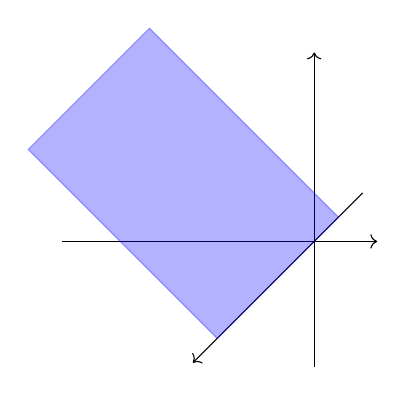
\begin{tikzpicture}[scale=0.8]
	\draw[->](-4,0,0)--(1,0,0); %y
    \draw[->](0,-2,0)--(0,3,0) ;%z
    \draw[->](0,0,-2)--(0,0,5) ;%x
      \filldraw[blue, opacity=0.3] (0,0,-1)--(-3,3,-1)--(-3,3,4)--(0,0,4)--cycle;
     
    
   % \draw[->, line width=2pt,red, -stealth](0,0,0)--(2,3,0);
    % \draw[->, line width=2pt,blue, -stealth](0,0,0)--(0,2,2.5);
    
\end{tikzpicture}

Is $V$ closed under scalar multiplication?
 
 \begin{multipleChoice}
 \choice{Yes}
 \choice[correct]{No}
 \end{multipleChoice}
 
 Is $V$ closed under addition?
 
 \begin{multipleChoice}
 \choice[correct]{Yes}
 \choice{No}
 \end{multipleChoice}
\end{problem}

\begin{problem} 
$V$ consists of all vectors along the line, as shown.

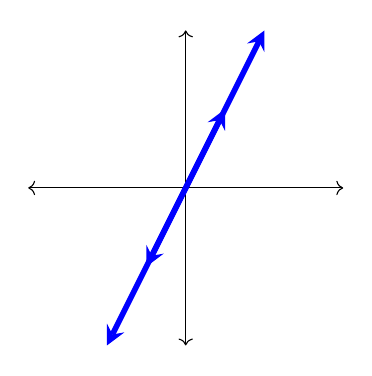
\begin{tikzpicture}[scale=0.5]

  \draw[<->] (-4,0)--(4,0);
  \draw[<->] (0,-4)--(0,4);
  \draw[->,line width=2pt,blue, -stealth] (0,0)--(2,4);
  \draw[->,line width=2pt,blue, -stealth] (0,0)--(-2,-4);
  \draw[->,line width=2pt,blue, -stealth] (0,0)--(1,2);
  \draw[->,line width=2pt,blue, -stealth] (0,0)--(-1,-2);
  
 \end{tikzpicture}
 
 Is $V$ closed under scalar multiplication?
 
 \begin{multipleChoice}
 \choice[correct]{Yes}
 \choice{No}
 \end{multipleChoice}
 
 Is $V$ closed under addition?
 
 \begin{multipleChoice}
 \choice[correct]{Yes}
 \choice{No}
 \end{multipleChoice}
\end{problem}    
\end{problem}

\begin{problem}\label{pr:opposite_in_subspace}
Prove Theorem \ref{opposite_in_subspace}.
\end{problem}

\begin{problem}\label{pr:null(A)_is_subspace}
Let $A$ be an $m \times n$ matrix.  Let $V$ be the subset of $\RR^n$ consisting of all vectors $\vec{x}$ such that $A \vec{x} = \vec{0}$.  Prove that $V$ is a subspace of $\RR^n$.  (Note that this subspace is called the null space of the matrix $A$ and we will denote it $null(A)$.)
\end{problem}

\end{document}
